% Contexte général - historique

Le sujet de TER porte sur la recherche d'un flot maximum dans un graphe quelconque par
l'utilisation d'algorithmes reposant sur la notion de \emph{préflot}, qui est une fonction obtenue
par relaxation des contraintes de la structure de flot. \\

\section{Un peu d'histoire}

Le problème de flot maximum, consistant à déterminer la quantité maximum de \emph{ressources} que
l'on peut transporter d'un point $A$ à un point $B$ dans un graphe, trouve ses racines, d'après A. 
Schrijver~\cite{schrij02} dans un rapport de Harris et Ross rédigé pour l'US
Air Force, en 1955, intitulé \emph{Fundamentals of a Method for Evaluating Rail Net Capacities}.  Il
s'agit là de la résolution d'un problème de flot maximum dans un graphe basé sur le réseau de
chemin de fer couvrant l'ouest de l'Union Soviétique et les pays satellites de l'Europe de l'est,
afin d'obtenir une coupe minimale de celui-ci, ce pour des raisons stratégiques.

Le problème fut ensuite étudié par Ford et Fulkerson qui rédigèrent un algorithme permettant de
résoudre le problème par l'utilisation de chaînes améliorantes dans le graphe, en 1955. De
nombreuses améliorations de l'algorithme ont vues le jour telles que l'algorithme d'Edmonds-Karp en
1969~\cite{gold88} ou l'algorithme de Dinic en 1970~\cite{gold88}, permettant, à l'aide d'une sélection 
judicieuse des chaînes améliorantes de réduire la complexité de l'algorithme initial.\\

\emph{Note : Il sera supposé, tout au long de ce document que le lecteur connaît ces derniers
algorithmes.} \\

% Problèmatique

Cependant, il existe de nombreux graphes pour lesquels l'exécution des algorithmes cités
ci-dessus est très longue. Le graphe représenté à la figure \ref{graphe_defaut} (p.
\pageref{graphe_defaut}) est l'un d'eux. C'est pour cette raison que la notion de préflot a été
développée, et aujourd'hui, les algorithmes basés sur les préflots font partie des plus rapides
développés à ce jour.\\

\begin{figure}[h!]
	\begin{center}
		\begin{tikzpicture}
			\tikzset{noeud/.style={circle, draw=black, text centered,minimum size=26pt, inner sep=0pt},
			fleche/.style={thick}};

			\node[noeud] (t) at (14, 0) {$t$};
			\node[noeud] (s) at (2, 0) {$s$};

			\foreach \x in {2, 3, 4, 5}{
				\node[noeud] (\x) at (2*\x, 0) {$\x$}; 
			}

			\foreach \y/\ytext in {3.5/6, 1.7/7, -1.7/n-2, -3.5/n-1}{
				\node[noeud] (\ytext) at (12, \y) {$\ytext$};
				\draw[fleche] (5) --node[right] {$1$} (\ytext) --node[left] {$1$} (t);
			}

% 	\foreach \y/\ytext in {-1.5/n-4, -3/n-3, -4.5/n-2, -6/n-1}{
% 		\node[noeud] (\ytext) at (14, \y) {$\ytext$};
% 		\draw[fleche] (6) to[bend right] (\ytext); 
% 		\draw[fleche] (\ytext) to[bend right] (t);
% 	}

			\node (point) at (12, 0) {$\vdots$};

			\draw[fleche] (s) --node[above] {$\infty$} (2) --node[above] {$\infty$} (3) --node[above] {$\infty$}
			(4) --node[above] {$\infty$} (5) ;

		\end{tikzpicture}
	\end{center}
	\caption{Graphe mettant en défaut les algorithmes de recherche de chaînes améliorantes}
	\label{graphe_defaut}
\end{figure}

L'algorithme d'Edmonds-Karp, recherchant une chaîne améliorante de plus court chemin dans le graphe,
effectue $(n-6)$ recherche de chaînes améliorantes et atteint son temps maximal d'exécution. Ce
problème se résout très vite à l'aide de préflots, ce que nous allons voir.

Au préalable, la notion de préflot sera définie\footnote{ainsi qu'un bref rappel de la notion de
flot}, puis le principe de chaque algorithme sera présenté, ainsi que la démonstration de leur
validité et leur borne de temps d'exécution. La dernière partie portera sur le détail des tests
effectués et sur le traitement des résultats\footnote{Les structures de données utilisées sont
présentées dans la documentation fournie}.

\section{Définitions}

\subsection{Quelques rappels sur les graphes}

Un graphe $G$ est défini par un ensemble de sommets noté $S$ et un ensemble d'arêtes notées
$A$\footnote{Il paraît important de faire remarquer que la définition d'un graphe non simple est
	parfaitement rigoureuse, si l'on rajoute à cette définition une fonction dite d'incidence notée
	$\gamma : A \rightarrow S \times S$ qui associe à chaque arête de $A$ un couple de sommets de
$S$.}, ainsi qu'un sommet source noté $s$ et un sommet puits $t$.\\

\textbf{\underline{Les notations utilisées dans les graphes :}}\\

Soit un sommet $i \in S$, le voisinage sortant (respectivement entrant) de $i$ sera noté $A^+(i)$
(resp. $A^-(i)$).\\
Soient $i, j \in S$, s'il existe une arête reliant $i$ à $j$ appartenant à $A$, cette dernière sera
notée $(i,j)$ et sa capacité $c(i,j)$.

\subsubsection{La notion de flot}

Dans un graphe $G (S, A)$, un flot $f$ de $G$ est une application $x : A \rightarrow \mathbb{N}$
vérifiant les conditions suivantes : 
		\begin{equation}
			\label{flot_1}
			\forall (i,j) \in A \qquad 0 \leq x(i,j) \leq c(i,j)\quad \mbox{ avec }x(i,j)\mbox{ la valeur du flot sur
			l'arête }(i,j)
		\end{equation} 
		\begin{equation} 
			\label{flot_2}
			\forall i \in S - \{s,t\},\quad \sum_{j \in A^+(i)} x(i,j) = \sum_{k \in A^-(i)} x(k,i)
		\end{equation}
		\begin{equation}
			\label{flot_3}
			f = \sum_{j \in A^+(s)} x(s,j) = \sum_{k \in A^-(t)} x(k, t)
		\end{equation}
Toute l'essence du problème étudié consiste en la maximisation de cette valeur.

\subsubsection{La notion de préflot}

Le préflot étant une fonction obtenue par relaxation de contraintes sur les flots, son
domaine de définition est donc le même : il s'agit d'une application $x : A \rightarrow \mathbb{N}$
respectant les contraintes suivantes :
		\begin{equation}
			\label{preflot_1}
			\forall (i,j) \in A \qquad 0 \leq x(i,j) \leq c(i,j)
		\end{equation}
		\begin{equation} 
			\label{preflot_2}
			\forall i \in S - \{s,t\},\quad \sum_{j \in A^+(i)} x(i,j) \leq \sum_{k \in A^-(i)} x(k,i)
		\end{equation}
		\begin{equation}
			\label{preflot_3}
			f = \sum_{j \in A^+(s)} x(s,j) \geq \sum_{k \in A^-(t)} x(k, t)
		\end{equation}
On introduit alors la valeur $e(i)$ représentant l'excédent de flot d'un noeud $i \in S$, elle est
définie comme la différence entre le préflot entrant dans un noeud et le préflot sortant de celui-ci
: \begin{equation}
	e(i) = \sum_{j \in A^+(i)} x(i,j) - \sum_{k \in A^-(i)} x(k,i)
\end{equation}
 On peut alors écrire l'inéquation (\ref{preflot_2}) de cette manière :
\begin{equation}ss
\forall i \in S - \{s,t\},\quad \sum_{j \in A^+(i)} x(i,j) = \sum_{k \in A^-(i)} x(k,i) + e(i)
\end{equation}
De la même manière, l'inéquation \ref{preflot_3} sera réécrite de la sorte :
\begin{equation}
\sum_{j \in A^+(s)} x(s,j) = \sum_{k \in A^-(t)} x(k, t) + \sum_{i \in S-\{s,t\}} e(i)
\end{equation}

Un sommet $i \in S$ ayant un excédent $e$ non nul : $e(i) > 0$ sera qualifié appelé sommet actif, on
dira aussi qu'il est débordant.

\subsubsection{La notion de réseau résiduel}

Soit un graphe $G(S, A)$, un flot $f$ et $i,j$ deux sommets e $G$. On dira que l'arête
$(i,j)$ appartiendra au réseau résiduel $A_f$ si et seulement si :
\begin{equation}
	 r(i,j) = c(i,j) - x(i,j) > 0
\end{equation}

On appelle alors $r(i,j)$ la capacité résiduelle de l'arête $(i,j)$. De plus la présence d'un flot
$f$ circulant sur l'arc $(i,j)$ de valeur $x(i,j)$ entraîne la présence d'une arête $(j,i)$
dans le réseau résiduel de capacité résiduelle $r(j,i) = x(i,j)$. 

\subsection{Quelques fonctions importantes}

\subsubsection{Les fonctions de potentiel}

Il est important de réaliser un point précis sur les fonctions de potentiel. Certaines des
démonstrations réalisées au cours de ce rapport se basent sur l'utilisation de ces fonctions.

Considérons une structure de données appelée $D_0$ sur laquelle sont effectuée des opérations
numérotées. Appelons $D_i$ la structure de données résultant de la $i^e$ opération. On appelle
fonction de potentiel, toute fonction $\Phi$ qui, à une structure de données $D_i$ associe un réel
appelé potentiel, noté $\Phi(D_i)$. Ce formalisme est décrit à la figure \ref{formal} (p.
\pageref{formal}).

\begin{figure}[h]
	\begin{center}
		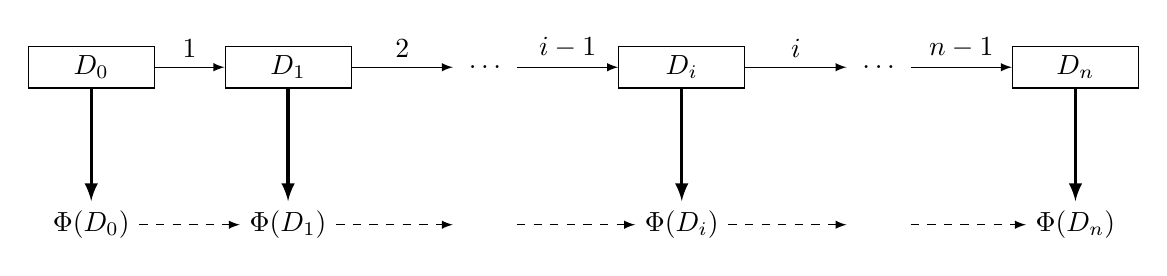
\begin{tikzpicture}
			\tikzset{noeud/.style={rectangle, draw=black, text centered, minimum width=16mm},
			nobud/.style={rectangle, text centered, minimum width=8mm}};
			\foreach \x/\xtext in {0/0, 1/1, 3/i, 5/n} {
				\node[noeud] (D\x) at (2.5*\x, 0) {$D_\xtext$};
				\node[nobud] (phi\x) at (2.5*\x, -2) {$\Phi(D_\xtext)$};
				\draw[->, very thick, >=latex] (D\x) to (phi\x);
			}
			\node[nobud] (ppp) at (5, 0) {$\dots$};
			\node[nobud] (ppp2) at (10, 0) {$\dots$};

			\node[nobud] (pp) at (5, -2) {$ $};
			\node[nobud] (p2) at (10, -2) {$ $};

			\draw[->, >=latex] (D0) --node[above] {$1$} (D1);
			\draw[->, >=latex] (D1) --node[above] {$2$} (ppp);
			\draw[->, >=latex] (ppp) --node[above] {$i-1$} (D3);
			\draw[->, >=latex] (D3) --node[above] {$i$} (ppp2);
			\draw[->, >=latex] (ppp2) --node[above] {$n-1$} (D5);

			\draw[->, >=latex, dashed] (phi0) -- (phi1);
			\draw[->, >=latex, dashed] (phi1) -- (pp);
			\draw[->, >=latex, dashed] (pp) -- (phi3);
			\draw[->, >=latex, dashed] (phi3) -- (p2);
			\draw[->, >=latex, dashed] (p2) -- (phi5);
		\end{tikzpicture}
	\end{center}
	\caption{Représentation du principe d'une fonction de potentiel}
	\label{formal}
\end{figure}

L'incidence de chacune des opérations sur la valeur de la fonction potentielle et la recherche d'une
borne supérieure à cette dernière permettra de déterminer des bornes sur le nombre d'opérations
effectuées et donc sur la complexité de l'algorithme.

\subsubsection{Fonction de distance}

Soit $G(S, A)$ un graphe ayant $s$ pour sommet source et $t$ pour sommet puits. Une fonction $d: S
\rightarrow \mathbb{N}$ est une fonction de hauteur\footnote{Aussi appelée \emph{fonction de
	hauteur}} si elle vérifie les propriétés suivantes :
\begin{subequations}
	\label{eq:prop_haut}
	\begin{align}
		d(s) &= |S| \label{eq:ph1} \\
		d(t) &= 0   \label{eq:ph2} \\
		\forall (i,j) \in A_f \quad d(i) &\leq d(j) + 1 \label{eq:ph3} 
	\end{align}
\end{subequations}

Une notion inhérente à la fonction de distance, est celle d'arête acceptable : une arête $(i,j)$ est
dite acceptable si et seulement si $d(i) = d(j) + 1$. Par définition, toute arête acceptable
appartient au réseau résiduel.

